\documentclass{ximera}
 

\usepackage{epsfig}

\graphicspath{
  {./}
  {figures/}
}

\usepackage{morewrites}
\makeatletter
\newcommand\subfile[1]{%
\renewcommand{\input}[1]{}%
\begingroup\skip@preamble\otherinput{#1}\endgroup\par\vspace{\topsep}
\let\input\otherinput}
\makeatother

\newcommand{\includeexercises}{\directlua{dofile("/home/jim/linearAlgebra/laode/exercises.lua")}}

%\newcounter{ccounter}
%\setcounter{ccounter}{1}
%\newcommand{\Chapter}[1]{\setcounter{chapter}{\arabic{ccounter}}\chapter{#1}\addtocounter{ccounter}{1}}

%\newcommand{\section}[1]{\section{#1}\setcounter{thm}{0}\setcounter{equation}{0}}

%\renewcommand{\theequation}{\arabic{chapter}.\arabic{section}.\arabic{equation}}
%\renewcommand{\thefigure}{\arabic{chapter}.\arabic{figure}}
%\renewcommand{\thetable}{\arabic{chapter}.\arabic{table}}

%\newcommand{\Sec}[2]{\section{#1}\markright{\arabic{ccounter}.\arabic{section}.#2}\setcounter{equation}{0}\setcounter{thm}{0}\setcounter{figure}{0}}

\newcommand{\Sec}[2]{\section{#1}}

\setcounter{secnumdepth}{2}
%\setcounter{secnumdepth}{1} 

%\newcounter{THM}
%\renewcommand{\theTHM}{\arabic{chapter}.\arabic{section}}

\newcommand{\trademark}{{R\!\!\!\!\!\bigcirc}}
%\newtheorem{exercise}{}

\newcommand{\dfield}{{\sf dfield9}}
\newcommand{\pplane}{{\sf pplane9}}

\newcommand{\EXER}{\section*{Exercises}}%\vspace*{0.2in}\hrule\small\setcounter{exercise}{0}}
\newcommand{\CEXER}{}%\vspace{0.08in}\begin{center}Computer Exercises\end{center}}
\newcommand{\TEXER}{} %\vspace{0.08in}\begin{center}Hand Exercises\end{center}}
\newcommand{\AEXER}{} %\vspace{0.08in}\begin{center}Hand Exercises\end{center}}

% BADBAD: \newcommand{\Bbb}{\bf}

\newcommand{\R}{\mbox{$\Bbb{R}$}}
\newcommand{\C}{\mbox{$\Bbb{C}$}}
\newcommand{\Z}{\mbox{$\Bbb{Z}$}}
\newcommand{\N}{\mbox{$\Bbb{N}$}}
\newcommand{\D}{\mbox{{\bf D}}}
\usepackage{amssymb}
%\newcommand{\qed}{\hfill\mbox{\raggedright$\square$} \vspace{1ex}}
%\newcommand{\proof}{\noindent {\bf Proof:} \hspace{0.1in}}

\newcommand{\setmin}{\;\mbox{--}\;}
\newcommand{\Matlab}{{M\small{AT\-LAB}} }
\newcommand{\Matlabp}{{M\small{AT\-LAB}}}
\newcommand{\computer}{\Matlab Instructions}
\newcommand{\half}{\mbox{$\frac{1}{2}$}}
\newcommand{\compose}{\raisebox{.15ex}{\mbox{{\scriptsize$\circ$}}}}
\newcommand{\AND}{\quad\mbox{and}\quad}
\newcommand{\vect}[2]{\left(\begin{array}{c} #1_1 \\ \vdots \\
 #1_{#2}\end{array}\right)}
\newcommand{\mattwo}[4]{\left(\begin{array}{rr} #1 & #2\\ #3
&#4\end{array}\right)}
\newcommand{\mattwoc}[4]{\left(\begin{array}{cc} #1 & #2\\ #3
&#4\end{array}\right)}
\newcommand{\vectwo}[2]{\left(\begin{array}{r} #1 \\ #2\end{array}\right)}
\newcommand{\vectwoc}[2]{\left(\begin{array}{c} #1 \\ #2\end{array}\right)}

\newcommand{\ignore}[1]{}


\newcommand{\inv}{^{-1}}
\newcommand{\CC}{{\cal C}}
\newcommand{\CCone}{\CC^1}
\newcommand{\Span}{{\rm span}}
\newcommand{\rank}{{\rm rank}}
\newcommand{\trace}{{\rm tr}}
\newcommand{\RE}{{\rm Re}}
\newcommand{\IM}{{\rm Im}}
\newcommand{\nulls}{{\rm null\;space}}

\newcommand{\dps}{\displaystyle}
\newcommand{\arraystart}{\renewcommand{\arraystretch}{1.8}}
\newcommand{\arrayfinish}{\renewcommand{\arraystretch}{1.2}}
\newcommand{\Start}[1]{\vspace{0.08in}\noindent {\bf Section~\ref{#1}}}
\newcommand{\exer}[1]{\noindent {\bf \ref{#1}}}
\newcommand{\ans}{}
\newcommand{\matthree}[9]{\left(\begin{array}{rrr} #1 & #2 & #3 \\ #4 & #5 & #6
\\ #7 & #8 & #9\end{array}\right)}
\newcommand{\cvectwo}[2]{\left(\begin{array}{c} #1 \\ #2\end{array}\right)}
\newcommand{\cmatthree}[9]{\left(\begin{array}{ccc} #1 & #2 & #3 \\ #4 & #5 &
#6 \\ #7 & #8 & #9\end{array}\right)}
\newcommand{\vecthree}[3]{\left(\begin{array}{r} #1 \\ #2 \\
#3\end{array}\right)}
\newcommand{\cvecthree}[3]{\left(\begin{array}{c} #1 \\ #2 \\
#3\end{array}\right)}
\newcommand{\cmattwo}[4]{\left(\begin{array}{cc} #1 & #2\\ #3
&#4\end{array}\right)}

\newcommand{\Matrix}[1]{\ensuremath{\left(\begin{array}{rrrrrrrrrrrrrrrrrr} #1 \end{array}\right)}}

\newcommand{\Matrixc}[1]{\ensuremath{\left(\begin{array}{cccccccccccc} #1 \end{array}\right)}}



\renewcommand{\labelenumi}{\theenumi)}
\newenvironment{enumeratea}%
{\begingroup
 \renewcommand{\theenumi}{\alph{enumi}}
 \renewcommand{\labelenumi}{(\theenumi)}
 \begin{enumerate}}
 {\end{enumerate}\endgroup}



\newcounter{help}
\renewcommand{\thehelp}{\thesection.\arabic{equation}}

%\newenvironment{equation*}%
%{\renewcommand\endequation{\eqno (\theequation)* $$}%
%   \begin{equation}}%
%   {\end{equation}\renewcommand\endequation{\eqno \@eqnnum
%$$\global\@ignoretrue}}

%\input{psfig.tex}

\author{Martin Golubitsky and Michael Dellnitz}

%\newenvironment{matlabEquation}%
%{\renewcommand\endequation{\eqno (\theequation*) $$}%
%   \begin{equation}}%
%   {\end{equation}\renewcommand\endequation{\eqno \@eqnnum
% $$\global\@ignoretrue}}

\newcommand{\soln}{\textbf{Solution:} }
\newcommand{\exercap}[1]{\centerline{Figure~\ref{#1}}}
\newcommand{\exercaptwo}[1]{\centerline{Figure~\ref{#1}a\hspace{2.1in}
Figure~\ref{#1}b}}
\newcommand{\exercapthree}[1]{\centerline{Figure~\ref{#1}a\hspace{1.2in}
Figure~\ref{#1}b\hspace{1.2in}Figure~\ref{#1}c}}
\newcommand{\para}{\hspace{0.4in}}

\renewenvironment{solution}{\suppress}{\endsuppress}

\ifxake
\newenvironment{matlabEquation}{\begin{equation}}{\end{equation}}
\else
\newenvironment{matlabEquation}%
{\let\oldtheequation\theequation\renewcommand{\theequation}{\oldtheequation*}\begin{equation}}%
  {\end{equation}\let\theequation\oldtheequation}
\fi

\makeatother

\begin{document}



\noindent In Exercises~\ref{c11.3.1a} -- \ref{c11.3.1b} use linear algebra to 
decide whether or not the origin is an asymptotically stable equilibrium for 
each system of ODEs $\dot{X}=AX$. If the origin is unstable, find an initial 
condition such that the corresponding solution approaches the origin as $t$ 
tends to infinity.  Verify these calculations using {\tt ode45}.
\begin{computerExercise} \label{c11.3.1a}
\begin{matlabEquation}\label{MATLAB:55}
A =  \left(\begin{array}{rrrr}
    -5  &  1  & -3  &  0\\
    -2  &  3  & -3  &  0\\
     4  & 11  & -5  &  0\\
     2  & -5  &  3  & -2
\end{array}\right)
\end{matlabEquation}

\begin{solution}

\ans The origin is a stable equilibrium.

\soln Create the following m-file to define the function {\tt exode4\_1}:
\begin{verbatim}
function f=exode4_1(t,x)
A = [-5     1    -3     0
     -2     3    -3     0
      4    11    -5     0
      2    -5     3    -2];
f = A*x;
\end{verbatim}
Compute the eigenvalues of $A$.  In this case, $\lambda_1 = -2$, $\lambda_2
\approx -0.25$, $\lambda_3 \approx -3.38 + 5.38i$, and $\lambda_4 \approx
-3.38 - 5.38i$ are eigenvalues of $A$.  All four eigenvalues have negative
real part, so the origin is a stable equilibrium.

\para To view the system using {\tt ode45}, choose an initial vector $X_0$
near the origin, and run {\tt ode45} using this vector.  Graphing the
components of the resulting $x$ confirms that all components converge on $0$
in forward time.  For example, the command
\begin{verbatim}
[t,x]=ode45('exode1',[0 5],[1,1,1,1]');
\end{verbatim}
runs {\tt ode45} on the system with initial vector $X_0 = (1,1,1,1)^t$.
The trajectories of the components of $x$ are shown in Figure~\ref{c11.3.1a}.

\begin{figure}[htb]
                       \centerline{%
                       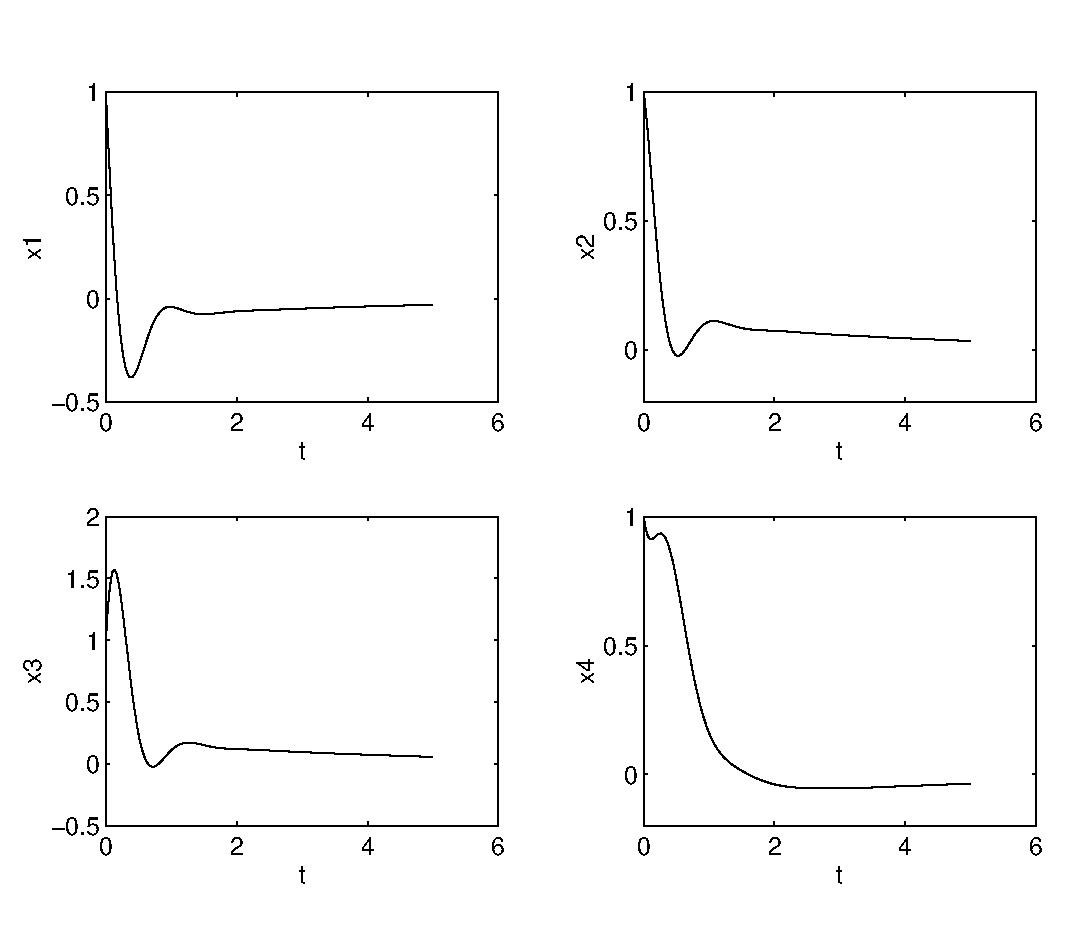
\psfig{file=exfigure/11-3-1a.eps,width=3.0in}}
                \exercap{c11.3.1a}
\end{figure}

\end{solution}
\end{computerExercise}
\begin{computerExercise} \label{c11.3.1b}
\begin{matlabEquation}\label{MATLAB:56}
A =  \left(\begin{array}{rrrr}
     0  &  1  & -3  &  0\\
    -2  &  3  & -3  &  0\\
     4  & 11  & -5  &  0\\
     2  & -5  &  3  & -2
\end{array}\right).
\end{matlabEquation}

\begin{solution}

\ans For the system $\dot{X} = AX$, the origin is not a stable
equilibrium, but for the initial condition $X_0 = (0,0,0,1)^t$, the
solution approaches the origin as $t$ tends to infinity.

\soln Create the m-file {\tt exode4\_2.m} corresponding to the system 
$\dot{X} = AX$:
\begin{verbatim}
function f = exode4_2(t,x)
A = [0     1    -3     0
    -2     3    -3     0
     4    11    -5     0
     2    -5     3    -2];
f = A*x;
\end{verbatim}
Compute the eigenvalues of $A$.  In this case, $\lambda_1 = -2$, $\lambda_2
= -2 + 6i$, $\lambda_3 = -2 - 6i$, and $\lambda_4 = 2$ are eigenvalues of
$A$.  In particular, $\lambda_4$ is positive and real, so the origin is not
a stable equilibrium for the system.

\para Confirm your results by choosing some initial vector, for instance,
$X_0 = (1,0,1,0)^t$ and computing its graph using {\tt ode45}.  Note that
values of the $x_i$ diverge as $t$ increases.
The trajectories of the components of $x$ are shown in Figure~\ref{c11.3.1b}. 

\para The eigenvalue $\lambda_1 = -2$ is negative and has
associated eigenvector $v = (0,0,0,1)^t$.  Run {\tt ode45} again, this
time with $X_0 = v$.  All solutions approach the origin.

\begin{figure}[htb]
                       \centerline{%
                       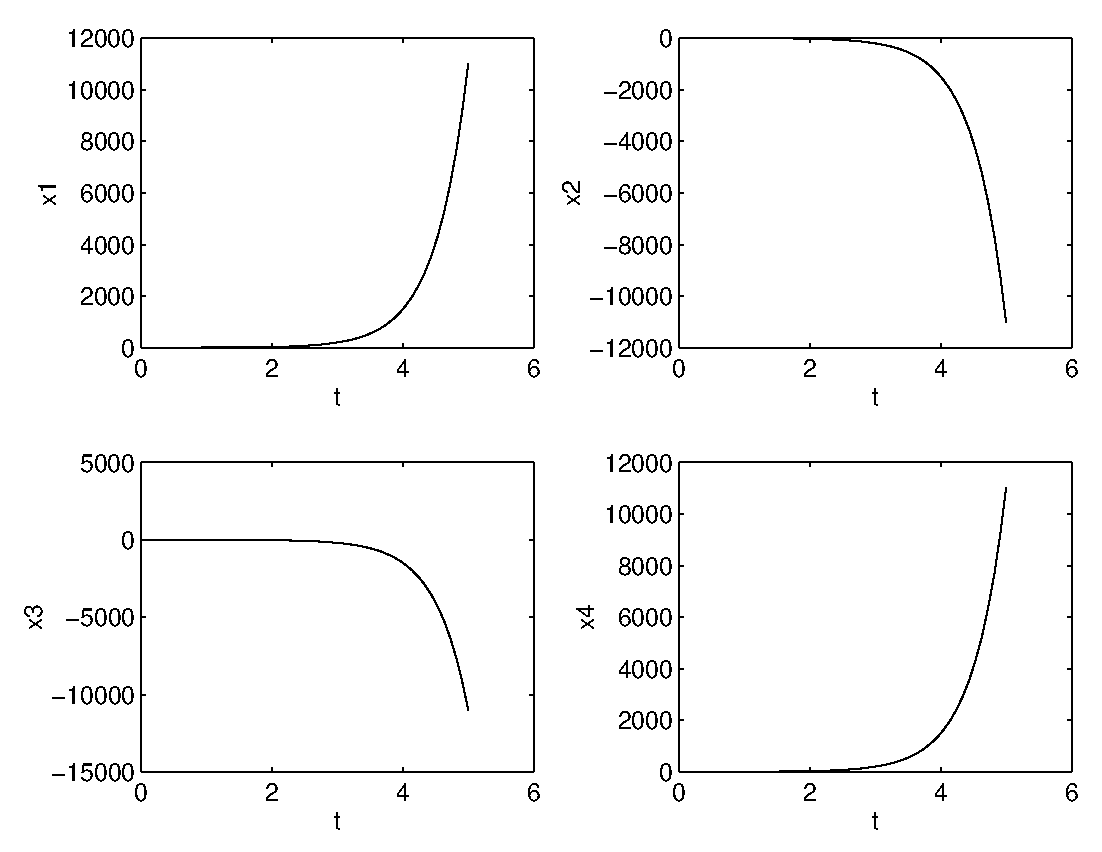
\psfig{file=exfigure/11-3-1b.eps,width=3.0in}}
                \exercap{c11.3.1b}
\end{figure}

\end{solution}
\end{computerExercise}
\end{document}
